% Picture at the beginning of the Set chapter

\def\firstcircle{(0,0) circle (3cm)}
\def\secondcircle{(0:4cm) circle (3cm)}

\colorlet{circle edge}{blue!50}
\colorlet{circle area}{blue!20}

\tikzset{filled/.style={fill=circle area, draw=circle edge, thick},
    outline/.style={draw=circle edge, thick}}

\begin{center}
% Set A and B
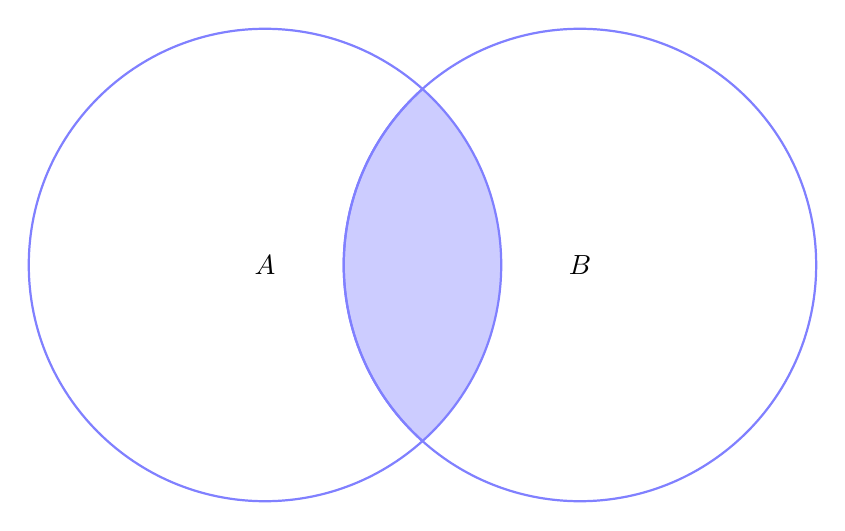
\begin{tikzpicture}
    \begin{scope}
        \clip \firstcircle;
        \fill[filled] \secondcircle;
    \end{scope}
    \draw[outline] \firstcircle node {$A$};
    \draw[outline] \secondcircle node {$B$};
    %\node[anchor=south] at (current bounding box.north) {$A \cap B$};
\end{tikzpicture}
\end{center}

